\begin{tmpfigure2}
    \neuripsonly{\vskip -0.5\baselineskip}
    \vskip -0.5\baselineskip
    \centering
    \begin{subfigure}[t]{0.48\textwidth}
        \centering
        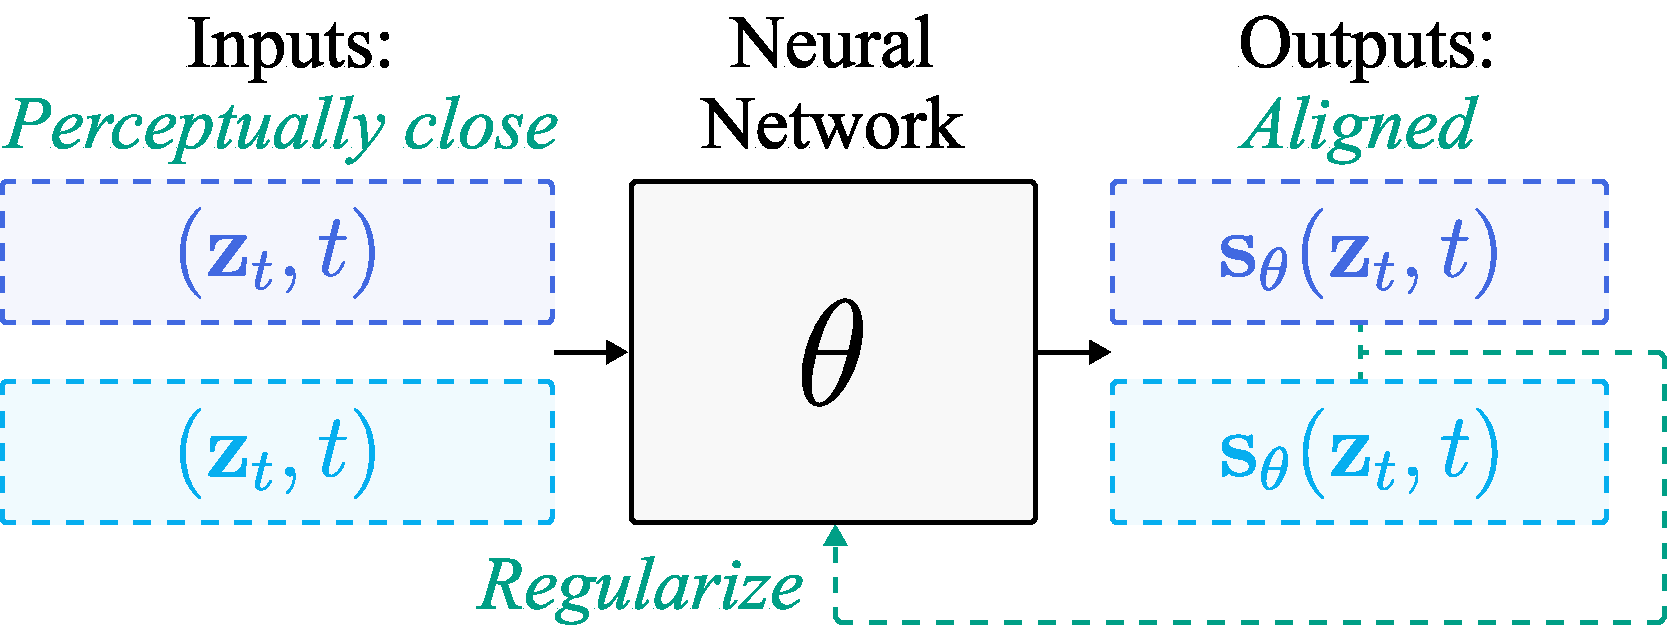
\includegraphics[width=\textwidth]{figures/performance/pat_def}
        \caption{\textbf{Definition of \xxgreen{PAT.}}}
        \label{fig:pat-def}
    \end{subfigure}
    \hfill
    \begin{subfigure}[t]{0.48\textwidth}
        \centering
        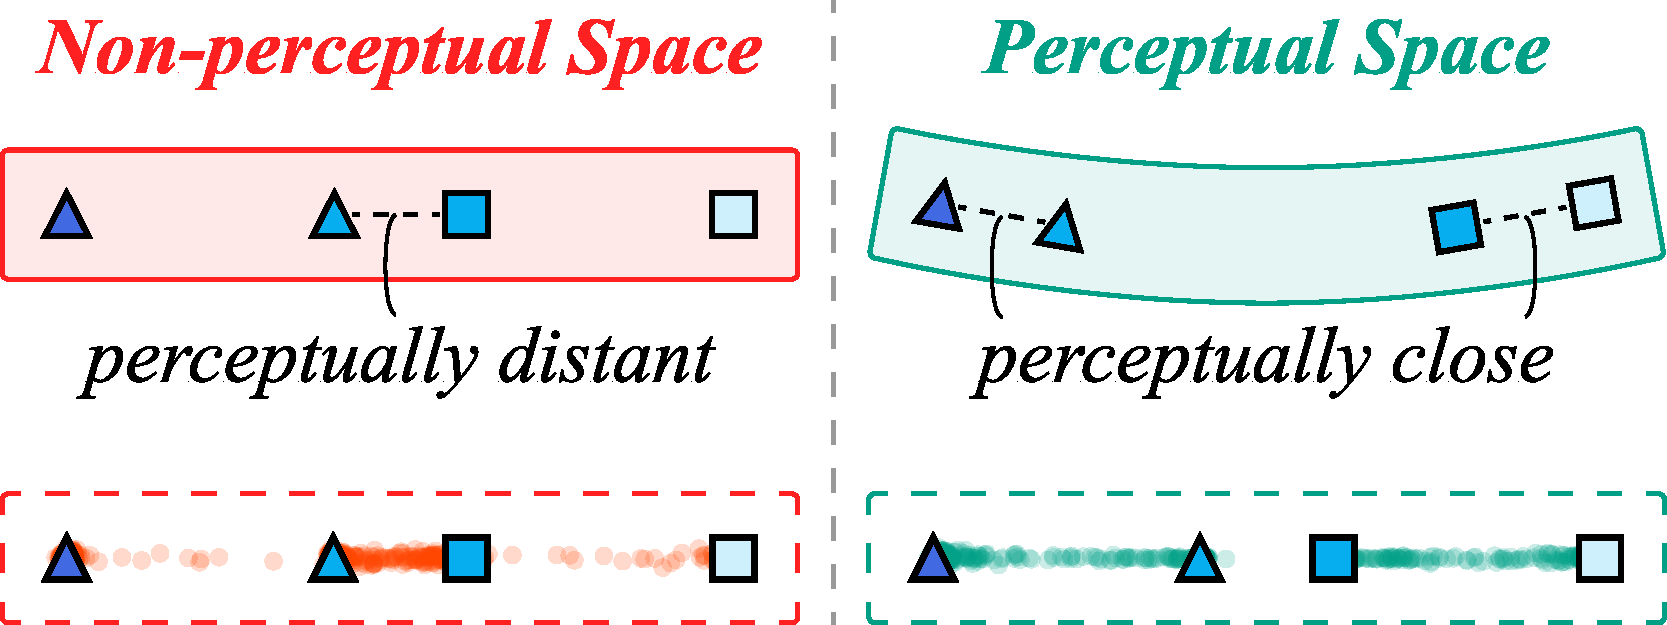
\includegraphics[width=\textwidth]{figures/performance/pat_space}
        \caption{\xblue{\textbf{Aligning diffusion space.}}}
        \label{fig:pat-space}
    \end{subfigure}
    \vskip 0.2\baselineskip
    \begin{subfigure}[t]{0.48\textwidth}
        \centering
        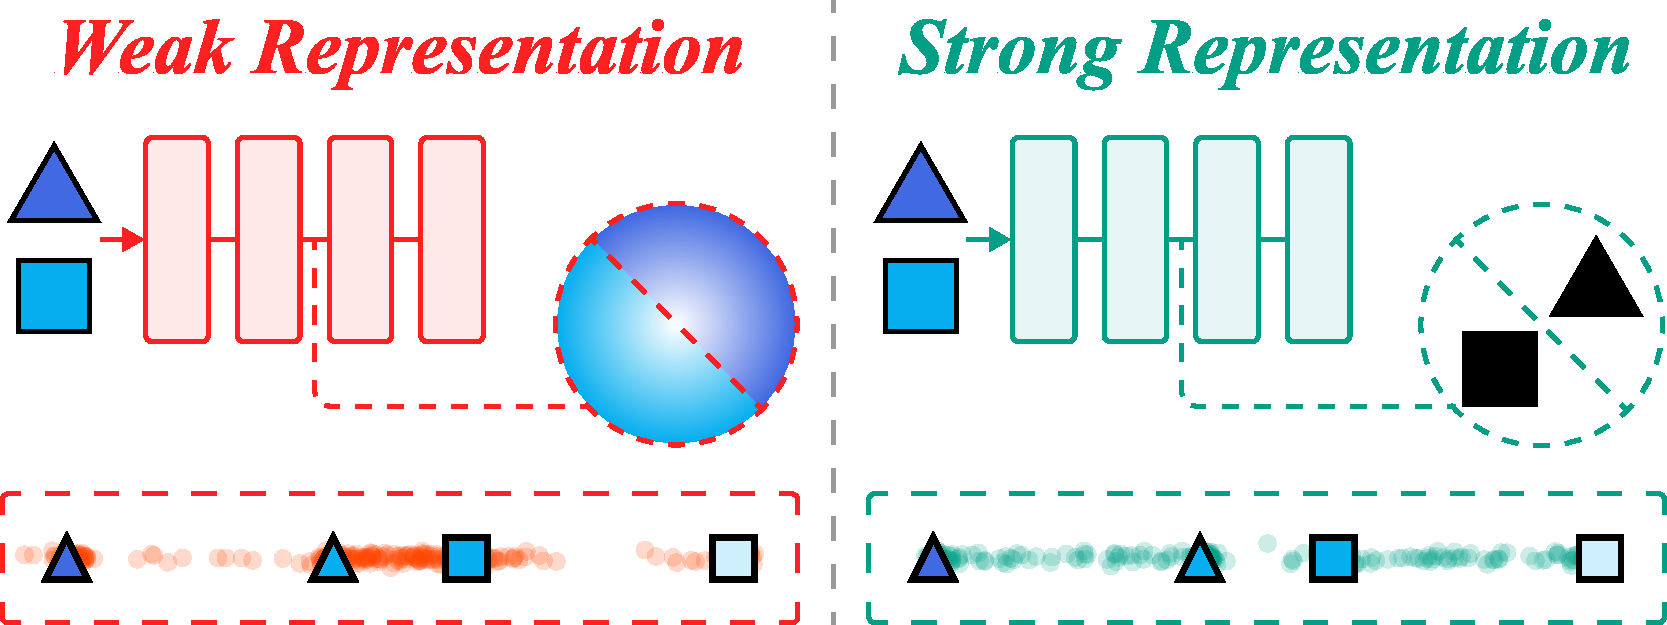
\includegraphics[width=\textwidth]{figures/performance/pat_representation}
        \caption{\xolive{\textbf{Aligning representation.}}}
        \label{fig:pat-representation}
    \end{subfigure}
    \hfill
    \begin{subfigure}[t]{0.48\textwidth}
        \centering
        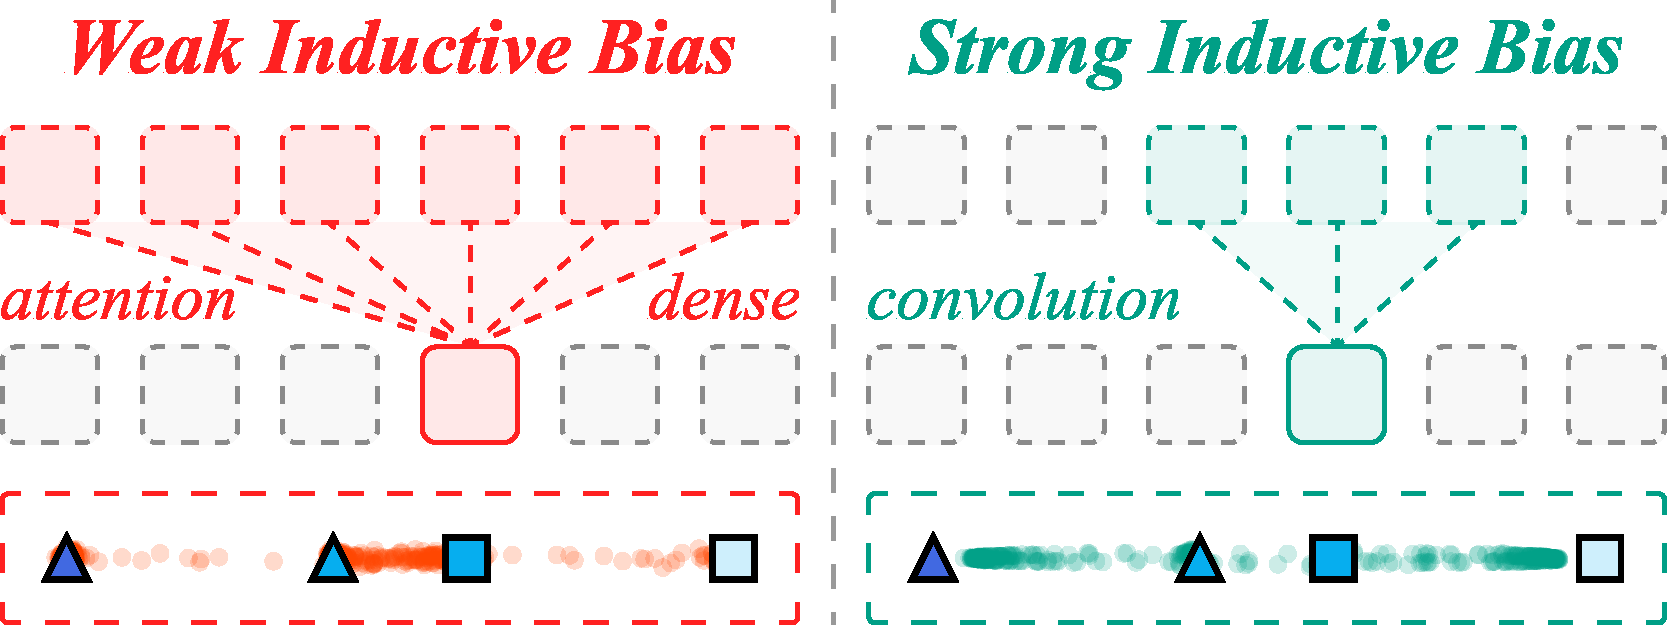
\includegraphics[width=\textwidth]{figures/performance/pat_architecture}
        \caption{\xxpurple{\textbf{Aligning architectural bias.}}}
        \label{fig:pat-architecture}
    \end{subfigure}
    \venueifelse{\vskip -0.5\baselineskip}{\vskip -0.25\baselineskip}
    \caption{\textbf{Illustration of \xxgreen{\emph{Perception-Aligned Training} (PAT)} with toy experiment results.}
    \xxgreen{PAT regularizes} a neural network $\theta$ to output \xxgreen{\emph{aligned}} scores $\rvs_\theta$ for \xxgreen{\emph{perceptually close}} inputs $\rvz_t$. Many successful training techniques can be unified under this view, categorized as the three instances.} \label{fig:pat}
    % For each: \emph{Top}, visual explanations; \emph{Bottom}, experiment results; \textbf{\emph{Left}, \coloreddashul{xred}{without PAT}; \emph{Right}, \coloreddashul{xxgreen}{with PAT}.}}
    \vskip -\baselineskip
\end{tmpfigure2}